\documentclass[a4paper, 11pt]{article}
\usepackage{graphicx} % Required for inserting images
\usepackage[portuguese]{babel}

\title{BD-PL01}
\author{Eduardo Fernandes}

\begin{document}

\maketitle

\noindent \textbf{Exercício 1}\\

\noindent A Dona Lucrécia é a rececionista de um escritório com muitos empresários. Várias encomendas chegam ao seu posto, e a Dona Lucrécia é responsável por as receber, para que um rapaz as possa distribuir pelos empresários.\\

\noindent Ultimamente, os empresários têm apresentado algumas queixas, a afirmar que não recebem encomendas que estavam à espera. Uma possível causa deste problema poderá ser os registos que a Dona Lucrécia tem efetuado, sendo que estes já se vêm a acumular durante os anos que ela trabalha no seu posto.\\

\noindent Para tal, a Dona Lucrécia decidiu criar uma pequena base de dados, que seja capaz de gerir os registos efetuados por esta.
Com a implementação do sistema de base de dados, a Dona Lucrécia espera atingir os seguintes objetivos:

\begin{itemize}
    \item melhorar a sua capacidade de gestão e registo das entregas;
    \item saber a qualquer momento as entregas já registadas;
    \item melhorar o controlo dos pagamentos efetuados;
    \item ...
\end{itemize}

\noindent Para criar este sistema, iremos trabalhar em conjunto com a Dona Lucrécia, para podermos criar uma lista de requisitos, que nos permita esquematizar a base de dados.\\

\newpage

\noindent \textbf{Exercício 2}\\

\noindent Lista de requisitos de Descrição:

\begin{itemize}
    \item cada \textbf{encomenda} é registada com um identificador único e o tipo de encomenda;
    \item cada \textbf{entregador} deve ser registado com um identificador único, nome e empresa de entregas para qual trabalha;
    \item cada \textbf{funcionário} da empresa deve ser registado com um identificador único, nome e o seu setor de trabalho;
    \item todos os \textbf{pagamentos} efetuados devem ser registados com um identificador único, valor a pagar e tipo de pagamento.
\end{itemize}

\noindent \textbf{Exercício 3}\\

\noindent Através dos requisitos de descrição estabelecidos acima, podemos desenhar o seguinte esquema conceptual:

\begin{figure}[h]
    \centering
    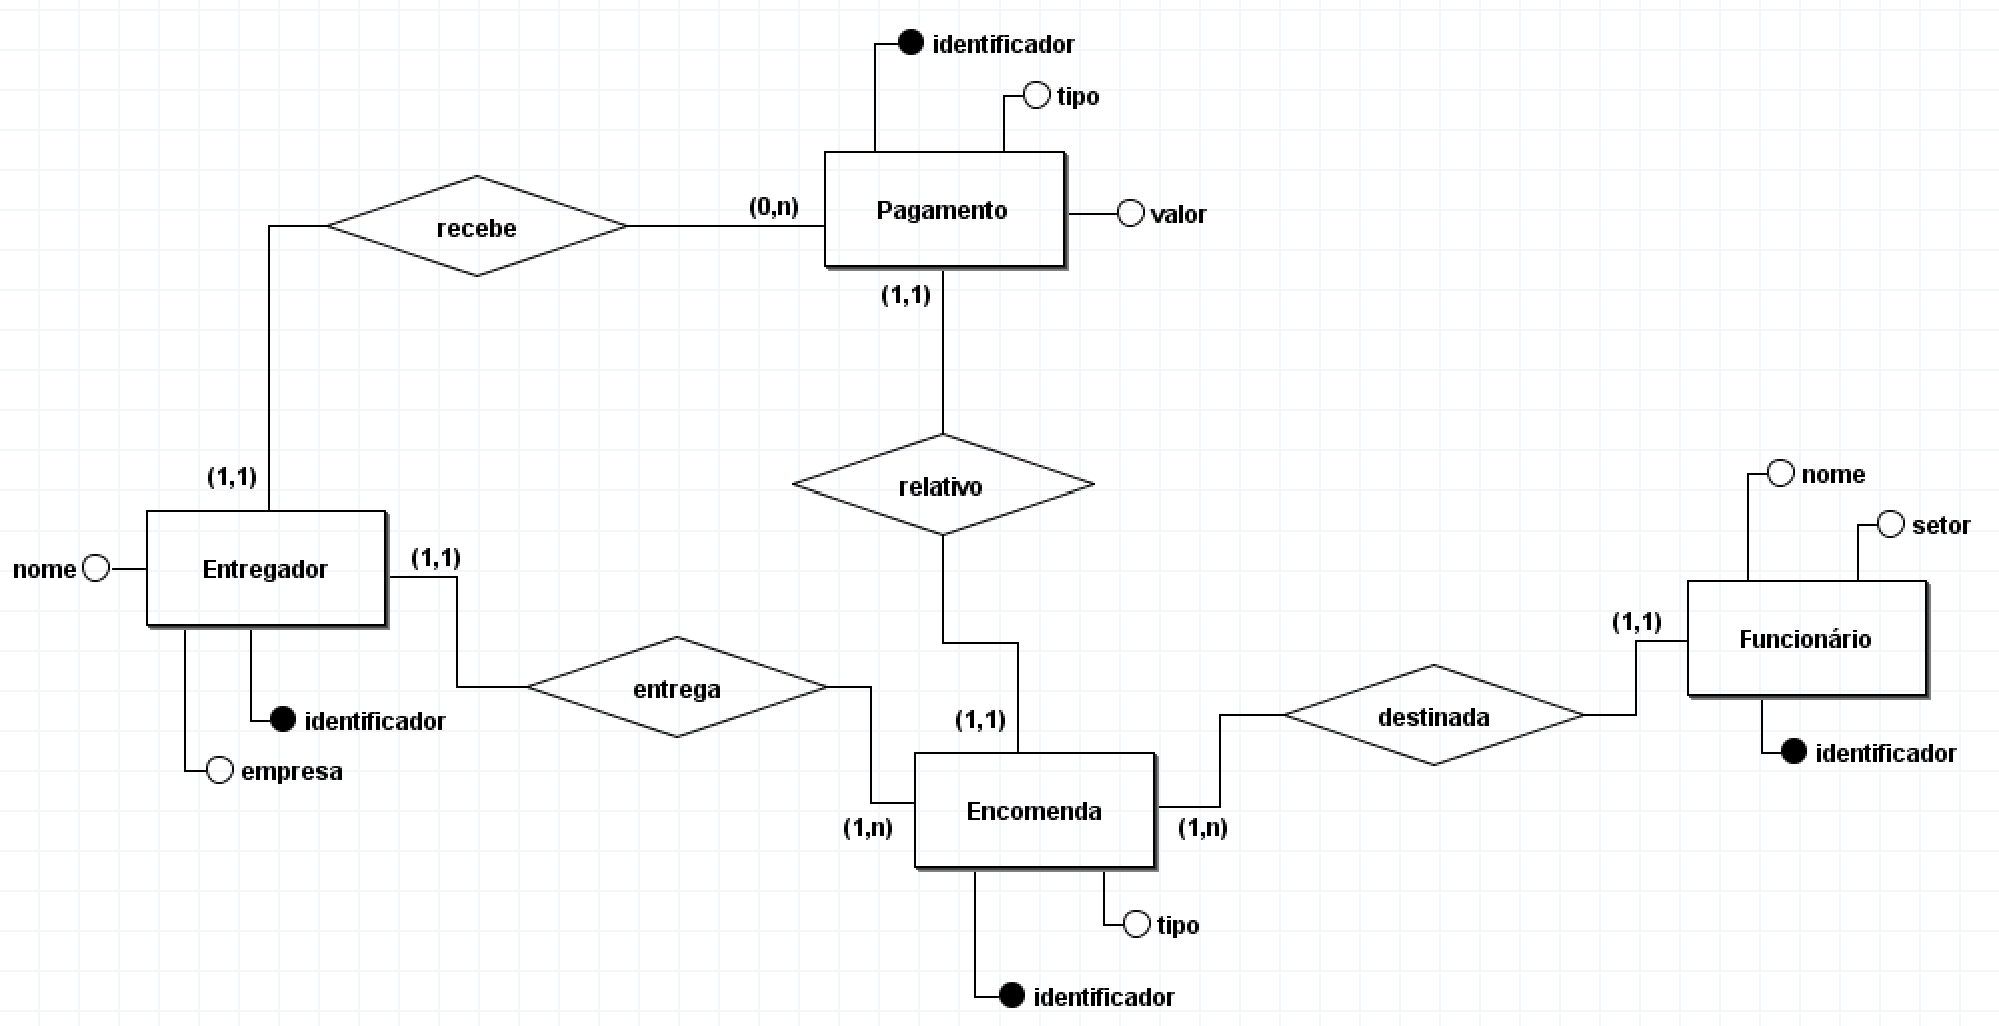
\includegraphics[width=1\linewidth]{modelo-pl01.png}
    \caption{Modelo Conceptual}
\end{figure}

\end{document}
